\chapter{Implementation and Results}
\label{cha:results}

\section{Implementation of EKF SLAM Algorithm}
\label{sec:slam_process}
The SLAM algorithm, as discussed in Chapter~\ref{cha:Overview}, consists of subparts each of which present challenges of its own. The primary purpose of this thesis is to develop a flexible implementation that can accommodate different algorithms for the subparts,hence, the guiding principle of the implementation is modularity. Hence an object oriented language such as Python is the platform of choice. This allows us to create individual objects for each part of the algorithm which can be substituted with ease to utilize different combinations of algorithms for feature extraction, association and filtering. 

During the initial setup, all the objects are created and initialized. A robot object is instantiated with its initial position and covariance representing the uncertainty in its position. This object holds the robot's position and uncertainty all through the runtime. It also contains objects for all the sensors and components that the actual robot contains. For example, an object of ENCODER class is instantiated with all its properties such as its noise factors, the diameter of the wheels it is attached on, and the separation between the wheels. A LIDAR object is also instantiated with the minimum and maximum range of the Hokuyo, the offset of the LIDAR from the center of the platform, and the measurement noise factors. These sensor objects are attached to the Robot object into proprioceptive and exteroceptive sensor lists, respectively. The proprioceptive sensors contain methods to calculate the motion model of the robot and also its Jacobian matrices.
To the exteroceptive sensors, feature extractor objects are attached. Each feature extraction algorithm is implemented as its own class. All such classes have to have a particular structure based on the sensor whose data the extractor uses. For LIDAR based extractors,  there has to be a function called \textit{get\_landmarks()} which takes in angles and distances and returns a list of landmark locations. They also need a member variable named \textit{landmarkType} which contains the type of landmark that the extractor is trying to find. 

The exteroceptive sensors are designed to take the list of landmark positions from each feature extractor attached to them and create objects of LANDMARK class for them. A combined list of landmark objects from all the feature extractors is returned by the exteroceptive sensor class. These landmark objects are objects of the LANDMARK class. This is a factory class which, for example, returns objects of either WALL or CYLINDER based on the \textit{landmarkType} returned by \textit{get\_landmarks}. Each of these classes contain methods to calculate their measurement models and their Jacobian matrices.
The main part of SLAM is carried out by an object of EKF class. This object contains  state and covariance members which represent the whole environment. In SLAM along with the robot's position being updated, the environment also needs to be mapped. So a representation of the environment called the map is held by an object of EKF class. It is essentially a list of all robot and landmark objects created.

\begin{figure}
\centering
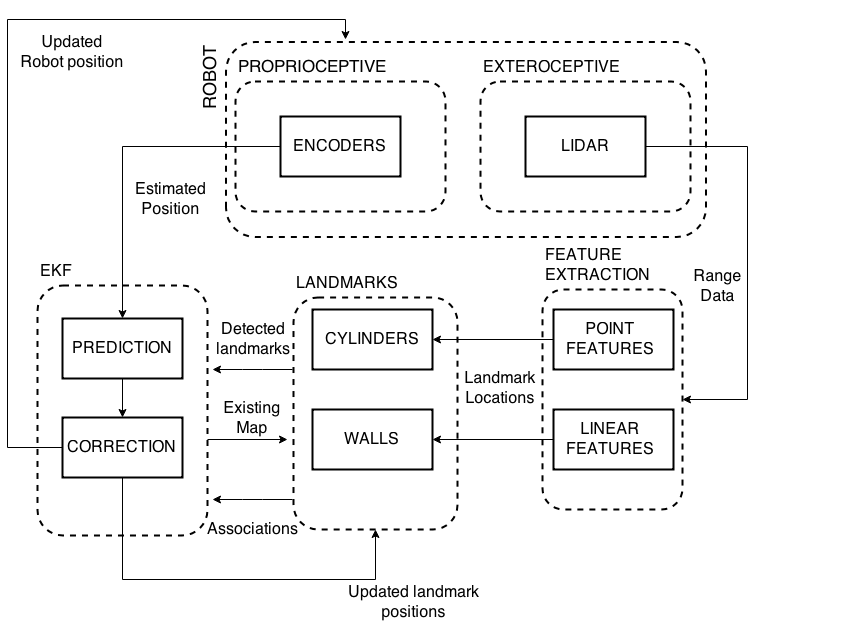
\includegraphics[width=\textwidth]{slam_process}
\caption{SLAM Implementation using only LIDAR.}
\label{fig:slam_process}
\end{figure}
Once initial setup is made, the robot object is added to the EKF map. Then for each time step, the \textit{run()} method of the EKF object is called. In this function the first step is prediction wherein for each robot in the map, the \textit{predict()} method of the robot object is called. That in turn calls the \textit{update()} method of all the proprioceptive sensors attached to that robot. This gives the estimated position and uncertainty using Equation~\ref{eq:Enc_3}. 

Then the \textit{observe()} method of the robot is called which in turn calls the exteroceptive sensors which generate landmark objects for all the landmarks seen at that time step. Each of these landmark objects are then checked to see if they are associated with a landmark preexisting in the map. For each re-observed landmark, the innovation and Kalman gain are calculated and the whole state is corrected. The map objects are then updated with the corrected positions. 

\section{Experimental Results}

To test the impact of the two feature extraction algorithms discussed in Chapter~\ref{cha:featureExtractor} on \slam, the \imp was driven around in first a controlled and then an uncontrolled indoor environment while continuously logging data. The Encoder and IMU data was logged at high speed at 100 Hz, and the LIDAR and Camera was logged at 5 Hz. The logged data was then analyzed using an EKF SLAM algorithm implemented as described in Section~\ref{sec:slam_process}. 

In the controlled environment, the two ends of a regular corridor are sealed off resulting in a closed space with no other features except walls and cylinders placed intentionally. This enables us to test the point feature extraction algorithm and see its effect on SLAM both individually and in combination with Hough transform based linear feature extraction. The controlled environment along with the path taken by IMP is seen in Figure~\ref{fig:overhead_path}. The closed-off space is still large enough such that it is not entirely within the range of the LIDAR. Hence, the problems and modifications discussed in Chapter~\ref{cha:featureExtractor} are still relevant even in a clean environment. 
\begin{figure}
\centering
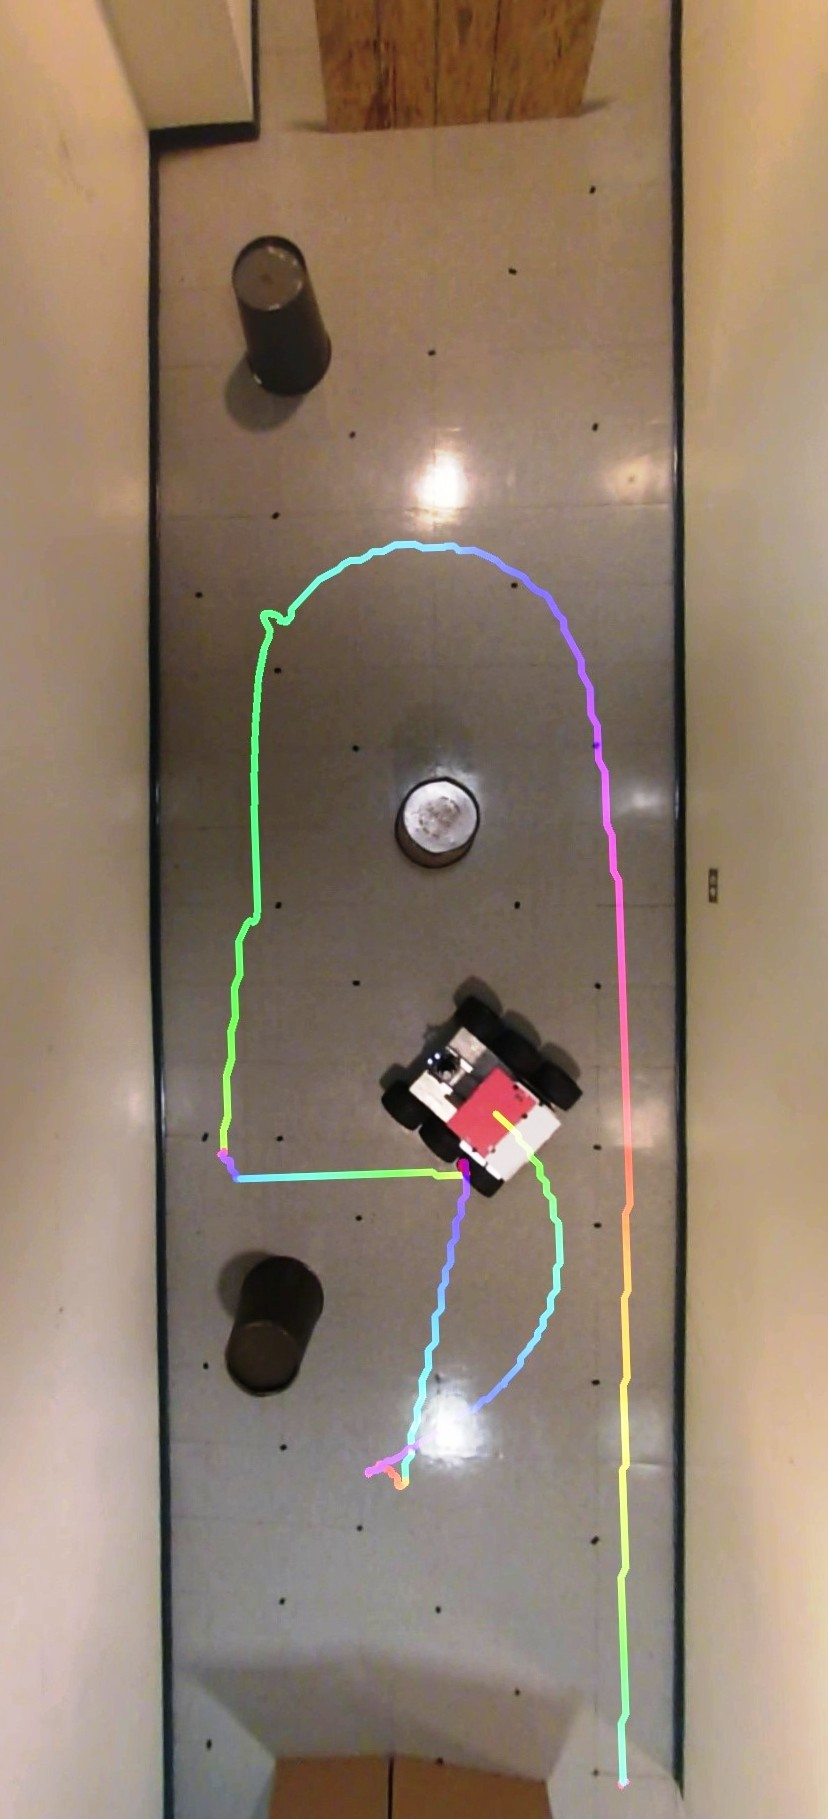
\includegraphics[height = 0.9\textheight]{overhead_path}
\caption{Controlled environment and path reconstructed by an overhead camera.}
\label{fig:overhead_path}
\end{figure}
To look at the effectiveness of the SLAM algorithm, some knowledge of the actual path taken by the robot is required for comparison. This is reconstructed using an overhead camera and the movement of the robot in the video is recorded. While this may not give the actual path or the ground truth accurately, it gives a reasonable estimate of it to within a few inches of deviation. A sample reconstructed path is shown in Figure~\ref{fig:overhead_path}. The camera based reconstructed path is also shown in all the plots of SLAM reconstructions for comparison. In the run, the robot starts at the bottom right corner and ends at the position shown.

Since the map is constructed relative to the starting location, the robot is always assumed to be starting at the origin in all the reconstructions.

\subsection{Using Point Features}
\label{sec: point_result}
In Figure~\ref{fig:overhead_path} the cylinders around which the robot travels are the point features that are to be detected. The algorithm used is the same as described in Section~\ref{sec: spikeAlgo}. Using just the jump in distance as a landmark results in a large number of spurious landmarks. As discussed in Section~\ref{sec: spikeAlgo}, it is therefore necessary to filter through the candidate landmarks using preexisting knowledge as previously described. The minimum number of points that need to be on the candidate landmark is chosen to be 11 for this particular arrangement. This is a tuning parameter which is decided after a few trials for optimized performance. The other tuning parameters include the thresholding for the range that the angular width can be in based on the radius of the cylinders which is $ 0.1524 $ m and the threshold for the curvature of the candidate landmark which is chosen to be $ 9 \% $. These tuning parameters are chosen only once for a particular environment. 

Once the feature extractor is tuned, the SLAM algorithm itself needs to be tuned based on the estimated noise factors for the various sensors. The SLAM algorithm is more robust to these parameters than the feature extractor and hence, a range of values yield good performance. Another part of the algorithm that needs to be tuned carefully is the landmark association. For point features in the map, the Euclidean distance between the detected and the preexisting cylinder is used. Hence, the maximum allowable distance for association needs to be set. That distance has to be large enough to accommodate for a particular landmark not being seen for a few steps and then being detected. It also should not be too large since this will result in wrong associations which will correct the path of the robot in a completely different way than the correct associations. Hence this parameter is also a function of the order of distances in the arena and is chosen to be $ 2 m $, in these experiments.
\begin{figure}
\centering
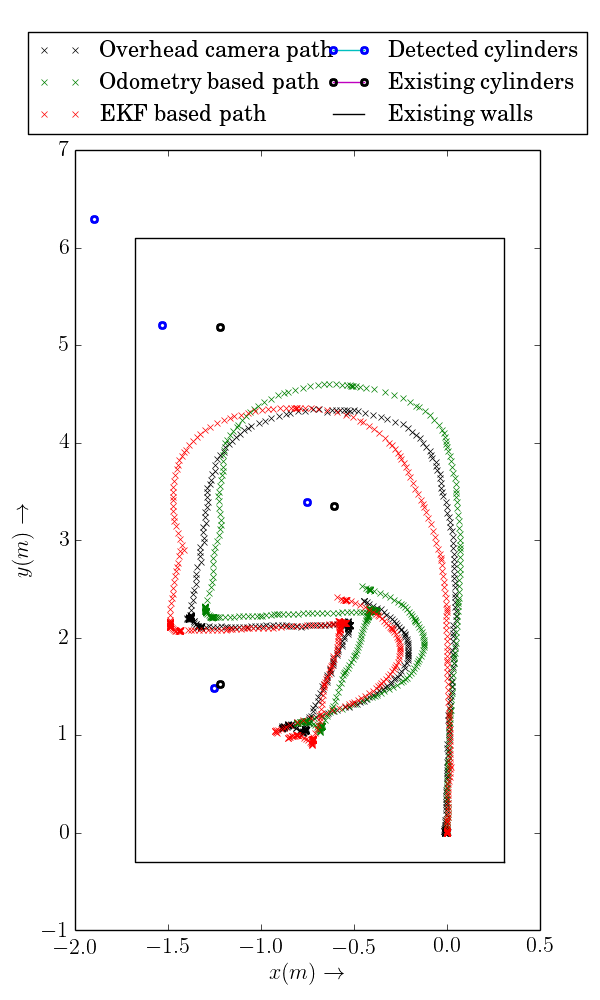
\includegraphics[height = 0.9\textheight]{cylinder}
\caption{Controlled environment and path reconstructed by detecting point features in LIDAR data. Path starts from the origin.}
\label{fig:cylinder_result}
\end{figure}

With these parameters, the path of the robot is reconstructed as seen in Figure~\ref{fig:cylinder_result}. We can see that it tries to correct the path towards the ground truth compared to the odometry based estimate, but it overcompensates frequently. This demonstrates the disadvantage of the conservative nature of the filters used. Since the focus is to not allow any spurious landmarks, the actual landmarks are also missed in a number of time steps. This effects the reconstruction mainly when there is only one landmark in the field of view of the LIDAR. 

In the part of the path that is shown in the upper right quadrant in Figure~\ref{fig:cylinder_result}, as soon as the robot has lost the first cylinder from its field of view, only the middle cylinder is seen for sometime until the robot turns and the third cylinder comes close enough to be resolved. This is the time interval when the SLAM reconstructed path deviates from the actual path as the heading was being previously corrected using the cylinders detected, but when the landmark is missed, the pure odometry keeps moving it in the same direction. A similar effect is seen in the upper right corner when the only cylinder that can be seen is the uppermost one. This compounds the error previously accumulated. It is only when the robot is able to see both the lower and the middle cylinders simultaneously, that the path is corrected. This overcompensation also results in a corresponding error in the reconstruction of the environment. This error as well as error in the end position of the robot is seen in Table~\ref{tab:cylinder_results}.

\begin{table}
\caption{Errors in environment reconstruction using point features.}
\label{tab:cylinder_results}
\begin{tabular}{| l | c | c | c |}
\hline ~ & Actual Position (x,y) & Detected Position (x,y) & Error(m)\\
\hline Cylinder 1 & (-1.2192,1.524) & (-1.2525,1.4851) & 0.002622 \\ 
\hline Cylinder 2 & (-0.6096,3.3528) & (-0.7522,3.3942) & 0.022048 \\ 
\hline Cylinder 3 & (-1.2192,5.1816) & (-1.5308,5.2055) & 0.097665 \\ 
\hline End Position & (-0.4459,2.3715) & (-0.5917,2.4141) & 0.023072 \\
\hline 
\end{tabular} 
\end{table}

\subsection{Using Linear Features}
\label{sec: hough_results}

In the controlled environment of Figure~\ref{fig:overhead_path}, the linear features are the 4 walls enclosing the space. For wall detection, two algorithms are discussed in Section~\ref{sec:extraction}. The RANSAC based algorithm, when implemented in the way discussed is seen to be not robust in Figure~\ref{fig: ransac_bad}. When used in SLAM it generates a number of spurious landmarks which result in wrong data association and subsequent correction. This results in the reconstruction being highly erroneous. 

Hence the Hough transform based algorithm is used. As described in Section~\ref{sec:hough}, the only tuning parameters for that algorithm are the pixel and angular resolution and threshold for line detection. Since these are broad parameters any reasonable value may be chosen. Since we use an image of 1000~$ \times $~1000 pixels to represent 10~m~$ \times $~10~m space in the real world, the physical significance of the pixel resolution is the minimum distance in centimeters that walls need to be far from each other for them to be considered as 2 individual walls instead of one. The angular resolution is useful as it avoids finding multiple walls with small angles between them. This is especially useful while reconstructing indoor environments as most walls tend to intersect at right angles hence corresponding to a very low probability that the actual line features intersect at a small angle. In this arena, an angular resolution of $ 10^\circ $ and a distance resolution of 2~cm is chosen. This allows a good reconstruction while speeding up the Hough transform itself as the size of the accumulator from Equation~\ref{eq:hough3} is reduced. 

\begin{figure}
\centering
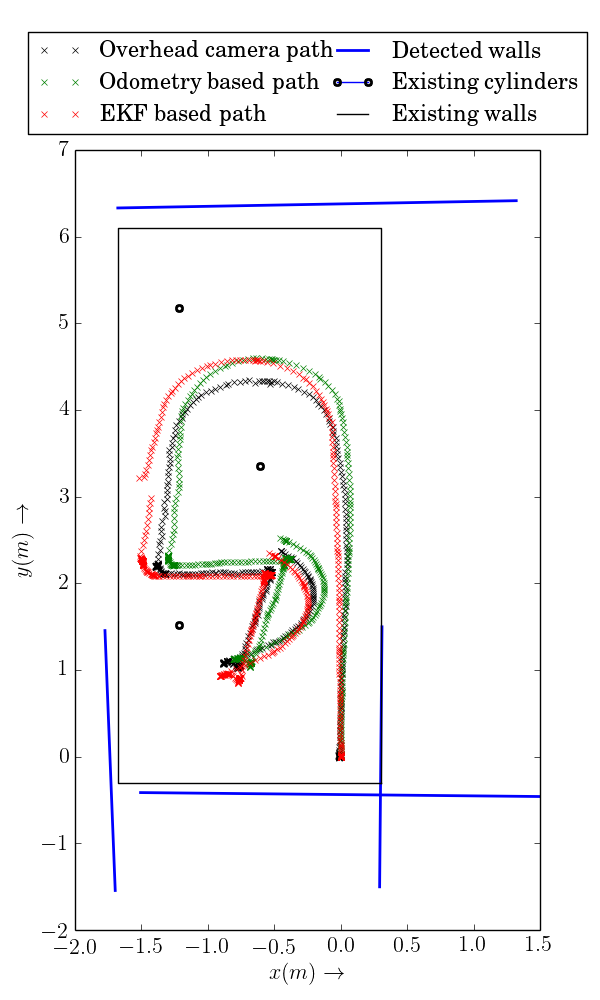
\includegraphics[height = 0.9\textheight]{walls}
\caption{Controlled environment and path reconstructed by detecting linear features in LIDAR data. Path starts from the origin.}
\label{fig:wall_result}
\end{figure}

The noise covariances for the encoder and LIDAR are kept the same as in Section~\ref{sec:Spike_results} since the same instruments are used. The only part that needs to be different from Section~\ref{sec: point_result} is the data association. There are a large number of ways that a linear feature can be associated. The simplest method is the Euclidean distance. This is feasible as the lines are represented in the normal form as shown in Figure~\ref{fig: normal_form}. Hence, the coordinates of the line are actually the point of intersection of the normal from the origin. If there is a difference in either angle or distance, the point of intersection will move. Hence the Euclidean distance between the detected and preexisting lines gives a good measure for association.

However, using solely the Euclidean distance is seen to have a drawback. It can lead to a wrong association when the lines are sufficiently close to the origin, such as in the bottom right corner of Figure~\ref{fig:overhead_path}. Then, the Euclidean distance between the points of intersection of the normals is lower than the threshold causing the 2 perpendicular walls to be associated as the same wall. Hence, it is necessary to add another heuristic to avoid this. The heuristic added in this implementation was based on the angle of intersection between the walls. The additional condition is that, even if Euclidean distance is small, if the angle of intersection is not close to 0 or 180 degrees, then the features are not associated with each other. With this addition, the path of the robot was reconstructed as shown in Figure~\ref{fig:wall_result}.


It is seen that the SLAM reconstruction is able to track the actual position for the most part except during the turn at the top and in a part close to the left wall. In the former case, the deviation from the path is mainly due to the odometry. This occurs as the robot has turned sufficiently to lose sight of the right wall and there are only small sections of the back and left wall in its field of view. This causes the walls to be not detected and emphasis is therefore, given to the odometry. In the part close to the left wall, the robot is moving slightly towards the wall in the ground truth whereas according to the odometry it is almost parallel. Since the only wall that the LIDAR can see at this point is the left wall and since the left wall has only recently been observed there is a greater tendency to move the estimated wall than the robot. This is also the reason in Figure~\ref{fig:wall_result}, for the left wall to be seen at an angle. Once the robot close enough to see the back wall, the SLAM reconstruction does a large correction resulting in the jump seen. The errors in the environment reconstruction as well as the path are shown in Table~\ref{tab:wall_results}. 

\begin{table}
\caption{Errors in environment reconstruction using linear features.}
\label{tab:wall_results}
\begin{tabular}{| l | c | c | c |}
\hline ~ & Actual Position (x,y) & Detected Position (x,y) & Error(m)\\
\hline Wall 1 & (0,-0.3048) & (-0.0066 -0.4371) & 0.017547 \\ 
\hline Wall 2 & (0.3048,0) & (0.3018,-0.0018) & 0.000012 \\ 
\hline Wall 3 & (0,6.096) & (-0.1784,6.3731) & 0.108611 \\ 
\hline Wall 4 & (-1.6764,0) & (-1.7358,-0.0447) & 0.005526 \\
\hline End Position & (-0.4459,2.3715) & (-0.5362,2.3477) & 0.008721 \\
\hline 
\end{tabular} 
\end{table}

\subsection{Using a Combination of Point and Linear Features}
\label{sec:combo_result}

As seen in Section~\ref{sec:slam_process}, the implementation of SLAM algorithm is designed to use both kinds of features simultaneously. With all the implementation details as in Sections~\ref{sec:Spike_results} and~\ref{sec: hough_results}, the reconstructed path is shown in Figure~\ref{fig:combo_result}.

\begin{figure}
\centering
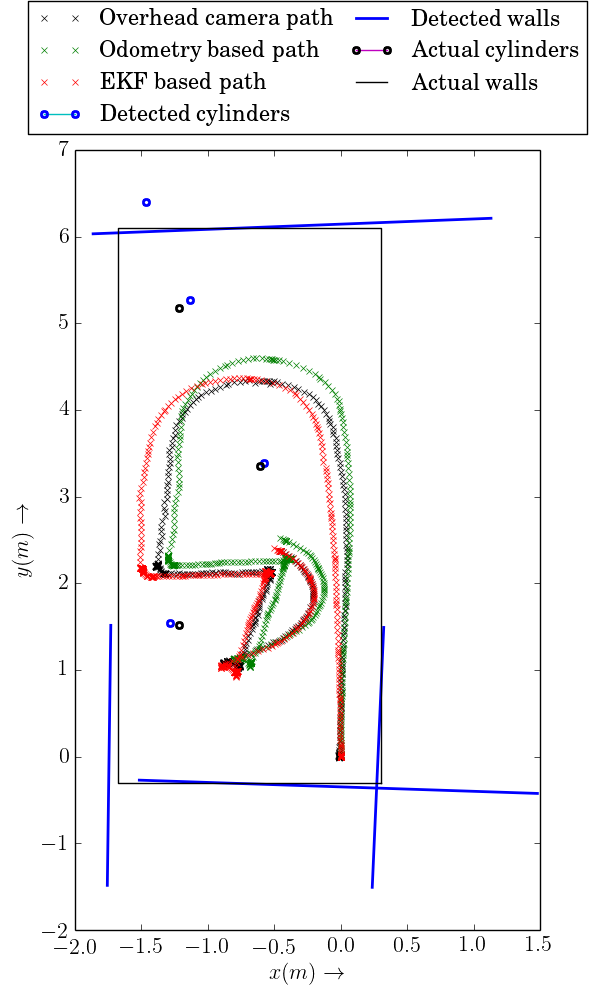
\includegraphics[height = 0.9\textheight]{both}
\caption{Controlled environment and path reconstructed by detecting both point and linear features in LIDAR data. Path starts from the origin}
\label{fig:combo_result}
\end{figure}


From the path, it is seen that a few of the errors from the previous two reconstructions have been corrected. For example, in Figure~\ref{fig:cylinder_result}, there is a large error in the top left part of the plot due to the cylinder not being detected robustly. In this path, the lack of the  cylinder feature is compensated for by using the walls. Since it is a corner region the algorithm is able to correct both position and orientation. In Figure~\ref{fig:wall_result}, there is a jump in the path near the left wall, and the left wall is reconstructed at an angle, as discussed in Section~\ref{sec: hough_results}. When the robot is traveling parallel to the left wall, it has 2 cylinders in its field of view, and hence, this jump is avoided.

There are still deviations from the path near the left wall as both the linear features based and the point features based reconstructions had both deviated at that region, a combination of the two cannot yield an accurate reconstruction, though it can be better than either one individually. The environment reconstruction errors are tabulated in Table~\ref{tab:combo_results}.

\begin{table}
\caption{Error in environment reconstruction using combination of linear and point features.}
\label{tab:combo_results}
\begin{tabular}{| l | c | c | c |}
\hline ~ & Actual Position (x,y) & Detected Position (x,y) & Error(m)\\
\hline Cylinder 1 & (-1.2192,1.524) & (-1.2856,1.5376) & 0.004602 \\ 
\hline Cylinder 2 & (-0.6096,3.3528) & (-0.5768,3.3911) & 0.002543 \\ 
\hline Cylinder 3 & (-1.2192,5.1816) & (-1.1308,5.2717) & 0.015932 \\
\hline Wall 1 & (0,-0.3048) & (-0.0177,-0.3476) & 0.002145 \\ 
\hline Wall 2 & (0.3048,0) & (0.2805,-0.0080) & 0.000654 \\ 
\hline Wall 3 & (0,6.096) & (-0.3663,6.1225) & 0.134878 \\ 
\hline Wall 4 & (-1.6764,0) & (-1.7436,0.0152) & 0.004747 \\
\hline End Position & (-0.4459,2.3715) & (-0.5013,2.4103) & 0.00457 \\
\hline 
\end{tabular} 
\end{table}

To compare the reconstructions, we can compare the landmark error values from the tables. In Table~\ref{tab:combo_results}, the total of all the cylinder errors is 0.0231 m. The corresponding errors in Table~\ref{tab:cylinder_results} add up to 0.1223 m. Hence, in terms of finding the location of the cylinders using the combination of both kinds of features reduces the error by 81.1\%. Similarly The total error in walls, for the combination of both is 0.142 and with just linear features is 0.132. Hence, using the combination of features is seen to increase the error, but only by 8\%. If we consider the end position of the robot, we see that compared to the point features based reconstruction, there is a 80\% reduction of error in the reconstruction using both types of features and a 47.5\% reduction compared to using only linear features. 

\subsection{Uncontrolled Environment with Linear Features}

\begin{figure}
    \centering
    \begin{subfigure}[b]{0.45\textwidth}
	    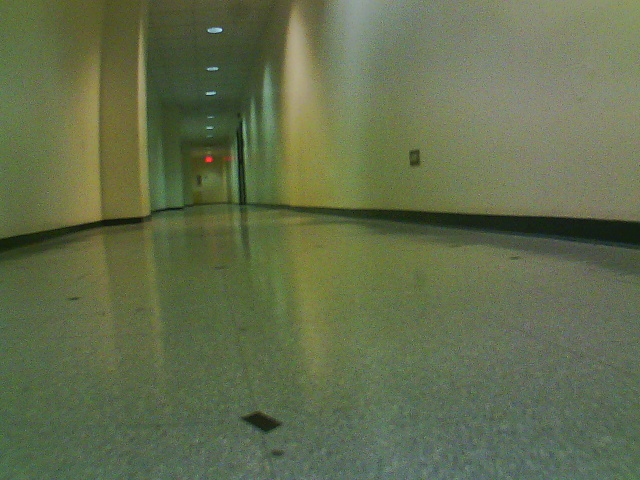
\includegraphics[width=\textwidth]{corr1}
    \end{subfigure}
    \quad %add desired spacing between images, e. g. ~, \quad, \qquad, \hfill etc.
      %(or a blank line to force the subfigure onto a new line)
    \begin{subfigure}[b]{0.45\textwidth}
        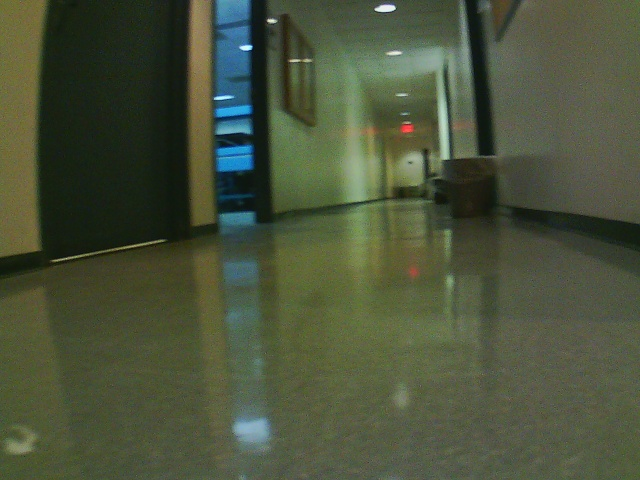
\includegraphics[width=\textwidth]{corr2}
    \end{subfigure}%

    \caption{Passages forming an uncontrolled environment.}
    \label{fig:onboard_1}
\end{figure}

\begin{figure}
    \centering
    \begin{subfigure}[b]{0.45\textwidth}
	    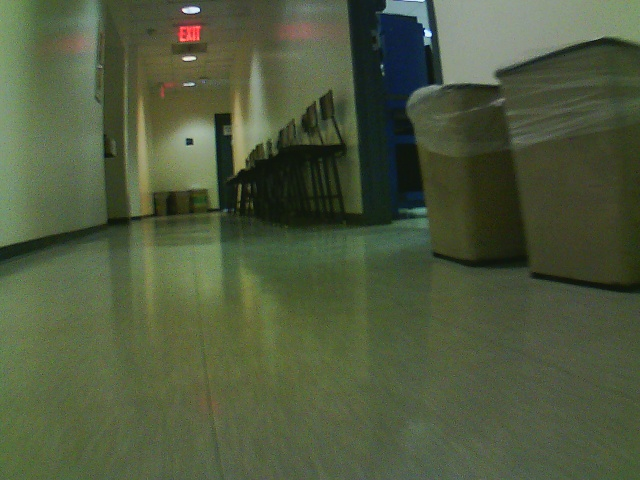
\includegraphics[width=\textwidth]{corr3}
    \end{subfigure}
    \quad %add desired spacing between images, e. g. ~, \quad, \qquad, \hfill etc.
      %(or a blank line to force the subfigure onto a new line)
    \begin{subfigure}[b]{0.45\textwidth}
        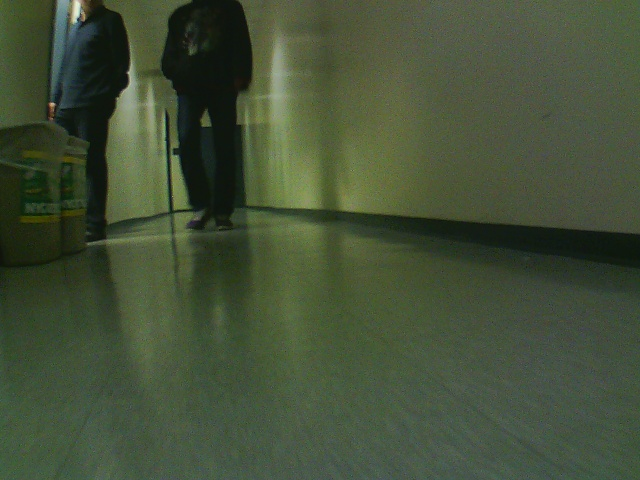
\includegraphics[width=\textwidth]{corr_human}
    \end{subfigure}%

    \caption{Obstacles in an uncontrolled environment.}
    \label{fig:onboard_2}
\end{figure}
The primary purpose of implementing EKF SLAM is to run it in real time. For this, it is essential that the tuning parameters previously discussed should not need to be tuned for each specific arena configuration. Hence, a longer run in an uncontrolled environment  with the same tuning parameters is analyzed.

From Section~\ref{sec:combo_result}, it is clear that the linear features based SLAM is relatively accurate compared to point features based SLAM. Although the combination of both walls and cylinders for SLAM gave the best results, the feature extractor for cylinder is seen to be conservative and not entirely robust. In Section~\ref{sec:hough}, it was shown that the Hough transform based linear feature extractor is robust to humans in its field of view. Hence for a long range uncontrolled indoor environment, the linear feature based SLAM is an ideal candidate. 

To test this, the robot is driven around a long passage which has both open and closed doors on either side as seen in Figure~\ref{fig:onboard_1}. There are also people walking around and entering and leaving through those doors. As seen in Figure~\ref{fig:onboard_2}, there are also other unintentional point features in the environment. 

This gives a challenge for both EKF based SLAM and for the Hough feature extractor. The correction should ideally be made based only on walls and not other lines such as door ways etc. For SLAM itself, since the distance traveled is much larger and the velocity with which the robot moves is also larger, the encoders drift by a considerable amount as seen in Figure~\ref{fig:big_run}. Since the run is in a larger environment, the ground truth is approximated manually, without any overhead camera data. It can be seen that linear feature based SLAM does a good job in estimating the path traveled compared to the odometry. It does not completely reconstruct the ground truth due to the large number of disturbances throughout it's path such as doors. Towards the end of the run, a number of estimated wall are seen due to the shape of the passages in that region. 

\begin{figure}
\centering
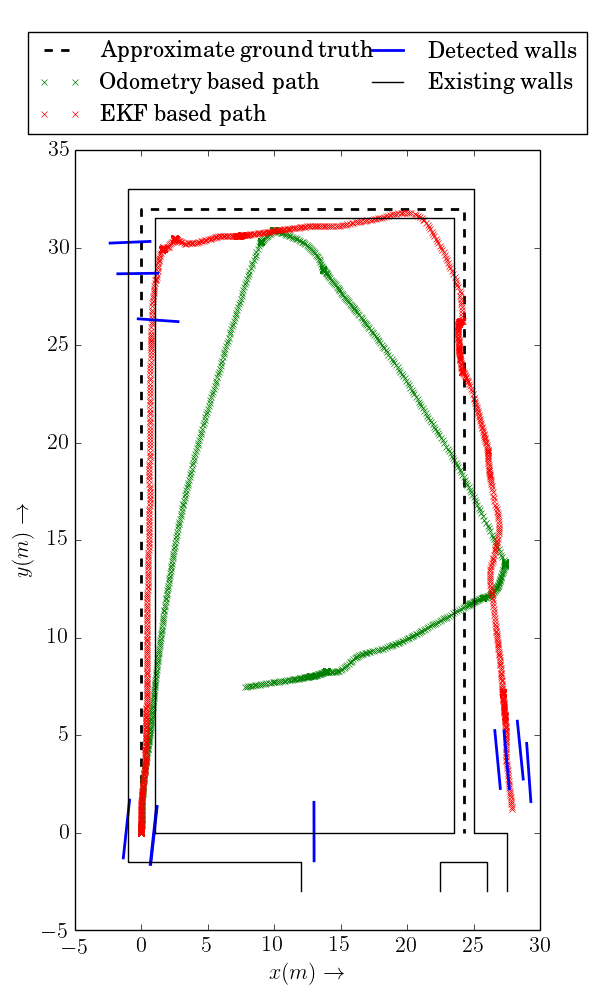
\includegraphics[height = 0.9\textheight]{big_run}
\caption{Uncontrolled environment and path reconstructed by detecting linear features in LIDAR data. Path starts from the origin.}
\label{fig:big_run}
\end{figure}

Hence, it is seen that in an uncontrolled environment, the Hough transform based linear feature detector performs well at reconstructing the path of the robot, even though the reconstruction of the environment is not accurate. It is also seen that the tuning parameters chosen in Sections~\ref{sec:Spike_results} and~\ref{sec: hough_results}, are robust and do not need to be changed for similar environments. 